\documentclass[12pt, twoside]{article}
%\documentclass[12pt, twoside]{article}
\usepackage[letterpaper, margin=1in, headsep=0.2in]{geometry}
\setlength{\headheight}{0.6in}
%\usepackage[english]{babel}
\usepackage[utf8]{inputenc}
\usepackage{microtype}
\usepackage{amsmath}
\usepackage{amssymb}
%\usepackage{amsfonts}
\usepackage[nomessages]{fp} %\FPeval{\var-name}{2*sin(pi/6)}
\usepackage{siunitx} %units in math. eg 20\milli\meter
\usepackage{yhmath} % for arcs, overparenth command
\usepackage{tikz} %graphics
\usetikzlibrary{quotes, angles, arrows, arrows.meta}
\usepackage{pgfplots}
\usepgfplotslibrary{fillbetween}
\pgfplotsset{compat=1.16}
\usepackage{graphicx} %consider setting \graphicspath{{images/}}
\usepackage{parskip} %no paragraph indent
\usepackage{enumitem}
\usepackage{multicol}
\usepackage{venndiagram}

\usepackage{fancyhdr}
\pagestyle{fancy}
\fancyhf{}
\renewcommand{\headrulewidth}{0pt} % disable the underline of the header
\raggedbottom
\hfuzz=2mm %suppresses overfull box warnings

\usepackage{hyperref}

\fancyhead[LO]{La Scuola d'Italia / Dr.\ Huson / IB Math 11 \\* 18 November 2026}
\fancyhead[RO]{\fbox{\begin{minipage}{6cm}\footnotesize Nickname:\\[0.5cm]\end{minipage}}}
\fancyfoot[C]{\thepage}

\begin{document}
\subsubsection*{4.1 Homework: Quadratic Functions}

Problems 1--4 without a calculator. Problem 5 uses your GDC.
A quadratic function can be written in three forms. Use these letters for
the coefficients, as IB questions do.

\begin{center}
\renewcommand{\arraystretch}{1.5}
\begin{tabular}{|l|l|l|}
\hline
Standard form & $f(x) = ax^{2} + bx + c$ & $y$-intercept $(0,\ c)$; \
axis $x = -\tfrac{b}{2a}$ \\
\hline
Vertex form & $f(x) = a(x - h)^{2} + k$ & vertex $(h,\ k)$ \\
\hline
Factored form & $f(x) = a(x - p)(x - q)$ & $x$-intercepts $(p,\ 0)$ and
$(q,\ 0)$ \\
\hline
\end{tabular}
\end{center}

\begin{enumerate}[itemsep=0.15cm]

%--- Problem 1: One quadratic in three forms: c, p, q, h, k as equations from the right form and a labelled sketch; axis by -b/2a; range; meaning of a and transformations from y = x^2; expand to check (last, on its own page) [15 marks] ---
%--- Source: Original (AA SL 2.6, 2.11); Haese AA SL Ch 2 ---
\item[1.]
The quadratic function $f$ can be written in three forms:
\[
f(x) = 3x^{2} - 12x - 15 \qquad
f(x) = 3(x - 2)^{2} - 27 \qquad
f(x) = 3(x + 1)(x - 5)
\]
\begin{enumerate}[itemsep=0.1cm]
  \item Choose the most useful form to write down each value. Write each
  answer as an equation, for example $a = 3$. Then sketch the graph of $f$
  on the grid, and label the $y$-intercept, the $x$-intercepts and the
  vertex.

  \noindent
  \begin{minipage}[t]{0.5\linewidth}
  \vspace{0pt}
  \begin{enumerate}[label=(\roman*), itemsep=0cm]
    \item the $y$-intercept, $c$
    \vspace{2.3cm}
    \item the $x$-intercepts, $p$ and $q$
    \vspace{2.3cm}
    \item the vertex, $h$ and $k$
  \end{enumerate}
  \end{minipage}%
  \begin{minipage}[t]{0.5\linewidth}
  \vspace{0pt}
  \begin{flushright}
  \begin{tikzpicture}[x=0.66cm, y=0.21cm]
    \draw [thin, color=gray, xstep=1, ystep=5] (-2.5,-30) grid (6.5,5);
    \foreach \x in {-2,-1,1,2,3,4,5,6}
      \draw[shift={(\x,0)}, color=black] (0pt,-2pt) -- (0pt,2pt) node[below] {\small $\x$};
    \foreach \y in {-30,-25,-20,-15,-10,-5,5}
      \draw[shift={(0,\y)}, color=black] (2pt,0pt) -- (-2pt,0pt) node[left] {\small $\y$};
    \draw [thick, ->] (-2.7,0) -- (6.9,0) node [right] {$x$};
    \draw [thick, ->] (0,-31) -- (0,6.5) node [right] {$y$};
    % solution curve: uncomment to check
    % \draw[thick, domain=-1.2:5.2, samples=60] plot (\x, {3*(\x-2)^2 - 27});
  \end{tikzpicture}
  \end{flushright}
  \end{minipage}

  \item Use $x = -\dfrac{b}{2a}$ to find the equation of the axis of
  symmetry. Check that the axis is halfway between the $x$-intercepts.
  \vfill
\end{enumerate}

\newpage

\begin{enumerate}[itemsep=0.1cm]
  \item[(c)] Write down the range of $f$. \vfill
  \item[(d)] State what the coefficient $a = 3$ tells you about the graph.
  Then describe two transformations that map the graph of $y = x^{2}$ onto
  the graph of $y = f(x)$. \vfill
  \item[(e)] Expand the vertex form and the factored form to show that each
  one equals $3x^{2} - 12x - 15$. \vfill \vfill
\end{enumerate}

\newpage

%--- Problem 2: Vertex form to standard and factored forms; sketch with intercepts and vertex; transformations from y = x^2 [12 marks] ---
%--- Source: Original (AA SL 2.6, 2.11); structure of AA SL 2021 Nov P1 Q1 with different numbers ---
\item[2.]
Let $g(x) = -(x - 1)^{2} + 9$.

\begin{enumerate}[itemsep=0.1cm]
  \item Write down the coordinates of the vertex. Is it a maximum or a
  minimum? \vfill
  \item Write $g(x)$ in the form $ax^{2} + bx + c$. \vfill \vfill
  \item Write $g(x)$ in the form $a(x - p)(x - q)$, and write down the
  $x$-intercepts. \vfill \vfill
\end{enumerate}

\noindent
\begin{minipage}[t]{0.45\linewidth}
\vspace{0pt}
\begin{enumerate}[itemsep=0.1cm]
  \item[(d)] Sketch the graph of $g$ on the grid. Label the vertex and the
  axis intercepts.
\end{enumerate}
\end{minipage}%
\begin{minipage}[t]{0.55\linewidth}
\vspace{0pt}
\begin{flushright}
\begin{tikzpicture}[scale=0.66]
  \draw [thin, color=gray, xstep=1.0cm, ystep=1.0cm] (-3.5,-1.5) grid (5.5,10.5);
  \foreach \x in {-3,-2,-1,1,2,3,4,5}
    \draw[shift={(\x,0)}, color=black] (0pt,-2pt) -- (0pt,2pt) node[below] {\small $\x$};
  \foreach \y in {-1,1,2,3,4,5,6,7,8,9,10}
    \draw[shift={(0,\y)}, color=black] (2pt,0pt) -- (-2pt,0pt) node[left] {\small $\y$};
  \draw [thick, ->] (-3.7,0) -- (5.9,0) node [right] {$x$};
  \draw [thick, ->] (0,-1.7) -- (0,10.9) node [right] {$y$};
  % solution curve: uncomment to check
  % \draw[thick, domain=-2.1:4.1, samples=60] plot (\x, {-(\x-1)^2 + 9});
\end{tikzpicture}
\end{flushright}
\end{minipage}

\newpage

\begin{enumerate}[itemsep=0.1cm]
  \item[(e)] Describe two transformations that map the graph of $y = x^{2}$
  onto the graph of $y = g(x)$. Give them in the correct order. \vfill
\end{enumerate}


%--- Problem 3: Signs of a, b, c and the discriminant from two unlabelled graphs [9 marks] ---
%--- Source: Original (AA SL 2.6, 2.7); standard IB Paper 1 format ---
\item[3.]
The diagrams show the graphs of two functions of the form
$y = ax^{2} + bx + c$.

\begin{center}
\begin{tabular}{cc}
\begin{tikzpicture}
\begin{axis}[axis lines=middle, xlabel={$x$}, ylabel={$y$},
  xtick=\empty, ytick=\empty, xmin=-2.5, xmax=4.8, ymin=-3, ymax=5.2,
  width=6.4cm, height=5.2cm, samples=100]
  \addplot[thick, domain=-1.2:4.2] {-(x-1.5)^2 + 4};
\end{axis}
\end{tikzpicture}
&
\begin{tikzpicture}
\begin{axis}[axis lines=middle, xlabel={$x$}, ylabel={$y$},
  xtick=\empty, ytick=\empty, xmin=-5.5, xmax=2.5, ymin=-1.5, ymax=6.5,
  width=6.4cm, height=5.2cm, samples=100]
  \addplot[thick, domain=-5.3:1.3] {0.5*(x+2)^2};
\end{axis}
\end{tikzpicture}
\\
Graph 1 & Graph 2
\end{tabular}
\end{center}

\begin{enumerate}[itemsep=0.1cm]
  \item Complete the table. Write \emph{positive}, \emph{negative} or
  \emph{zero} in each cell.

  \begin{center}
  \renewcommand{\arraystretch}{2.4}
  \begin{tabular}{|l|p{2.4cm}|p{2.4cm}|p{2.4cm}|p{2.4cm}|}
  \hline
   & $a$ & $b$ & $c$ & $\Delta = b^{2} - 4ac$ \\
  \hline
  Graph 1 & & & & \\
  \hline
  Graph 2 & & & & \\
  \hline
  \end{tabular}
  \end{center}
  \item Explain how you decided the sign of $b$ for Graph 1. \vfill \vfill
\end{enumerate}

\newpage

%--- Problem 4: Equation of a parabola from its intercepts and one point; standard form; vertex; range [9 marks] ---
%--- Source: Original (AA SL 2.6); standard IB "find the quadratic from its graph" format ---
\item[4.]
The graph of a quadratic function crosses the $x$-axis at $(-1,\ 0)$ and
$(5,\ 0)$, and the $y$-axis at $(0,\ 10)$.

\begin{enumerate}[itemsep=0.1cm]
  \item Find the equation of the graph in the form $y = a(x - p)(x - q)$.
  \vfill
  \item Write the equation in the form $y = ax^{2} + bx + c$. \vfill
  \item Find the coordinates of the vertex, and write down the range of the
  function. \vfill
\end{enumerate}

\newpage

%--- Problem 5 (GDC): revenue and cost curves, break-even points by graph intersection; profit interval; profit function; maximum profit [10 marks] ---
%--- Source: Original (AA SL 2.4, 2.6); market context from DP1_markets-and-functions_plan_2026-11 ---
\item[5.]
\emph{Use your GDC in this problem. Write down what you entered, and give
answers correct to three significant figures.}

A company makes $x$ hundred bicycle lights per week. Its weekly revenue $R$
and weekly cost $C$, both in thousands of euros, are modelled by
\[
R(x) = 40x - 2x^{2} \qquad \text{and} \qquad C(x) = 6x + 75,
\qquad 0 \le x \le 20.
\]

\begin{enumerate}[itemsep=0.1cm]
  \item Graph $y = R(x)$ and $y = C(x)$ on your GDC. Find the
  coordinates of the two points where the graphs intersect. These are the
  \emph{break-even} points. \vfill
  \item Write down the values of $x$ for which the company makes a
  profit. \vfill
  \item The profit is $P(x) = R(x) - C(x)$. Write $P(x)$ in the form
  $ax^{2} + bx + c$. \vfill
  \item Find the number of bicycle lights the company should make each
  week to earn the maximum profit, and find this maximum profit in euros.
  \vfill
\end{enumerate}

\end{enumerate}
\end{document}
